% !TEX root = ../Seminararbeit-Data_Mining_Frameworks.tex
%


% =============================================================================
%
% Der Data Mining Prozess
%
% =============================================================================
\chapter{Der Data Mining Prozess}
\label{sec:process}

Der Prozess des Data Minings lässt sich grundsätzlich durch die folgenden Phasen
beschreiben:
\begin{enumerate}
\item Sammeln von Daten: \\
Für das Sammeln von Daten ist unter Umständen spezielle Hardware, bspw.
Sensoren, händische Arbeit wie das Sammeln von Umfragebögen oder Software in
Form einer Webanwendung mit auszufüllenden Formularfeldern, notwendig. Auch wenn
diese Phase sehr Anwendungsspezifisch ist und oft vom Daten-Analysten nicht
beeinflusst werden kann, ist sie ausschlaggebend für das Ergebnis des Data
Mining Prozesses.
\item Bereinigen der Daten: \\
Oftmals sind die gesammelten Rohdaten aufgrund des Dateiformats oder einer
fehlenden Struktur nicht direkt verarbeitbar. Deshalb ist es wichtig, die Daten
in ein Format zu bringen, welches von Data Mining Algorithmen gelesen werden
kann.
\item Analyse der Daten: \\
Der letzte Schritt ist die Daten analytisch zu verarbeiten und Methoden zu
entwickeln, um diese nutzbar zu machen. Dies geschieht durch das Anwenden von
bestimmten Data Mining Algorithmen, welche für die jeweilige Aufgabenstellung
angepasst werden müssen.
\end{enumerate}
Um einen Standard für einen solchen Data Mining Vorgang zu etablieren, haben
einige große Unternehmen wie Automobilhersteller Daimler-Benz, Versicherungs
Provider OHRA, Hard- und Software Hersteller NCR Corp. und Statistik-Software
Hersteller SPSS Inc. den „CRoss-Industry Standard Process for Data Mining“
(kurz: CRISP-DM) definiert.

\pagebreak

\section{CRISP-DM}
\label{sec:process:crispdm}

\begin{figure}[htb]
	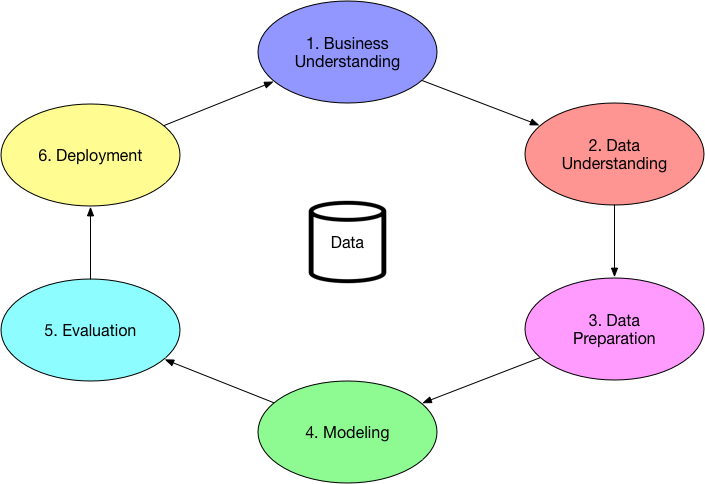
\includegraphics[width=\textwidth]{gfx/CRISP-DM_Model.png}
	\caption{Konzeptionelles CRISP-DM Modell}
	\label{fig:process:crispdm}
\end{figure}

\subsection{Business Understanding}
\label{sec:process:crispdm:bu}

Im ersten Schritt des CRISP-DM Prozesses, dem sog. Business- (oder auch Organizational-) Understanding,
ist es zunächst wichtig festzulegen was man mit dem Minen von Daten erreichen
möchte bzw. welche Informationen von Interesse sind. Hier findet auch eine oft
zitierte Textstelle aus Alice im Wunderland Anwendung:
\begin{quotation}
  >>Willst du mir wohl sagen, wenn ich bitten darf, welchen Weg ich hier nehmen muß?<< \\
  >>Das hängt zum guten Teil davon ab, wohin du gehen willst,<< sagte die Katze. \\
  >>Es kommt mir nicht darauf an, wohin –<< sagte Alice. \\
  >>Dann kommt es auch nicht darauf an, welchen Weg du nimmst,<< sagte die Katze. \\
  >>– wenn ich nur irgendwo hinkomme,<< fügte Alice als Erklärung hinzu. \\
  >>O, das wirst du ganz gewiß,« sagte die Katze, »wenn du nur lange genug gehest.<<
\end{quotation}
Konkret bedeutet das, dass es keine Rolle spielt wie lange man Daten Mined, wenn
man nicht festgelegt hat welche Informationen man gerne hätte. Es müssen also
zunächst Fragen festgelegt werden, welche durch das Data Mining beantwortet
werden sollen. Beispielsweise möchte man gerne wissen warum sich Kunden so sehr
beschweren, wie man die Profit-Spanne seiner Produkte vergrößert oder wie man
Fehler bei der Herstellung antizipieren kann.

\subsection{Data Understanding}
\label{sec:process:crispdm:du}



\subsection{Data Preparation}
\label{sec:process:crispdm:dp}

\subsection{Modeling}
\label{sec:process:crispdm:mod}

\subsection{Evaluation}
\label{sec:process:crispdm:eval}

\subsection{Deployment}
\label{sec:process:crispdm:depl}

\section{Alternativen}
\label{sec:alt}
